%!TEX root=../report.tex
\chapter{Test suite}\label{chp:test_suite}

The experiments that are going to be proposed aim at reproducing network configurations that are plausible on real distributed systems. Some of them are specifically crafted for causing troubles to the consensus algorithms taken into consideration and may seem far from typical real-life scenarios. Extreme network problems, such as multiple link failures, node crashes and network partitioning, indeed frequently happen.\\
The consensus algorithms have been analysed from different points of view. They have been firstly investigated to understand which of them overall performs best in a noise-free scenario. This test also provides the gold standard measure for each implementation to be taken into consideration for every successive comparison. Another key aspect has been the robustness of the consensus algorithms when the underlying network was suffering from problems. Extensive tests have been executed to understand how the system behaves when the network performances degrade gradually.\\
Before describing every test, it is worth underlying some peculiarities of the considered implementations. Multi-paxos suffers from unexpected crashes (with a probability of \(\sim0.005\%\)), especially when filters are applied by netem on the underlying network layer. The test daemon has retried failed operations until no exception was thrown. Particular attention has been paid to RethinkDB in order to obtain results consistent with respect to the other implementations. More specifically, caching mechanisms have been disabled on every node and operations have been configured to use the strongest available consistency level by using appropriate parameters during the API calls. In this way RethinkDB has been forced to reach consensus for every operation and to store the results on persistent storage, as Raft requires. A read operation has been executed after every write to ensure data was really replicated across the cluster. With these constraints test results were comparable with those gathered on other implementations. Google Datastore has been used in an improper way to some extent. The web-service is specifically designed to work best when batching lot of operations into a single request rather than sequentially uploading small objects, as it was done during the tests. Finally, some problems were encountered running PySyncObj on physically different machines. Due to these limits, tests of this implementation have not been performed on Compute Engine clusters.

\section{Tuning the number of operations}
Before running the test suite, the number of operations to perform had to be defined. Such value had to be chosen carefully in order to obtain statistically significant results. To tune it properly, the followed approach consisted of:

\begin{itemize}
    \item running twice one algorithm in a normal network environment for a determined number of operations;
    \item computing the cumulative distribution function (CDF) of the times collected in the previous step;
    \item comparing the CDFs;
    \item increasing the number of operations if CDFs were too different or validating the same number on another implementations otherwise.
\end{itemize}

The correctness of this approach can be justified by the frequentist definition of probability.
In the \enquote{long run}, as the number of trials approaches infinity, the relative frequency will converge exactly to the true probability, as stated by the following formula:

\[ 
P(x < t) = \lim_{nTot\to\infty} \frac{Nx}{nTot}
\]

where \(Nx\) represents the number of operations where the completion time is lower than \(t\).\\
Consequently, assuming that the underlying distribution remains the same, the two curve will both converge to the same originating cumulative distribution function. If two CDFs are similar enough no further investigation is needed, since more operations will only produce more similar distributions to those already computed, adding no significance to the tests. As it is possible to see from the experiments depicted in \ref{rethinkdb_stable} run on RethinkDB, 5000 has been proved to be a reasonably large value. 

\begin{figure}[H]
  \makebox[\textwidth][c]{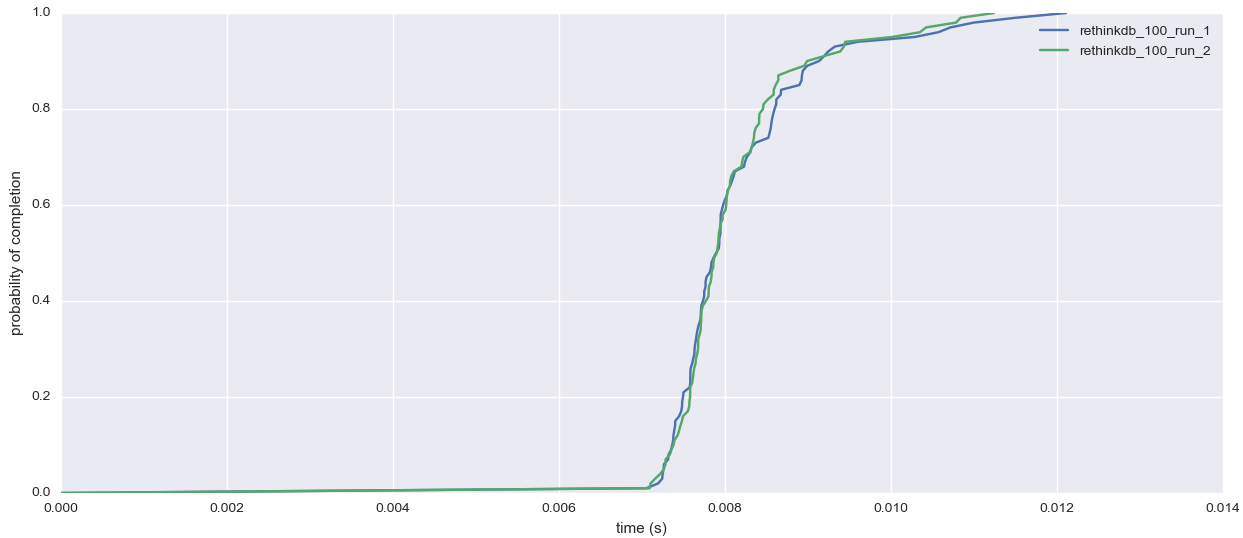
\includegraphics[width=0.8\paperwidth]{results_rethinkdb_100_mass.png}}
  \caption{RethinkDB: 100 run.}
\end{figure}

\begin{figure}[H]
  \makebox[\textwidth][c]{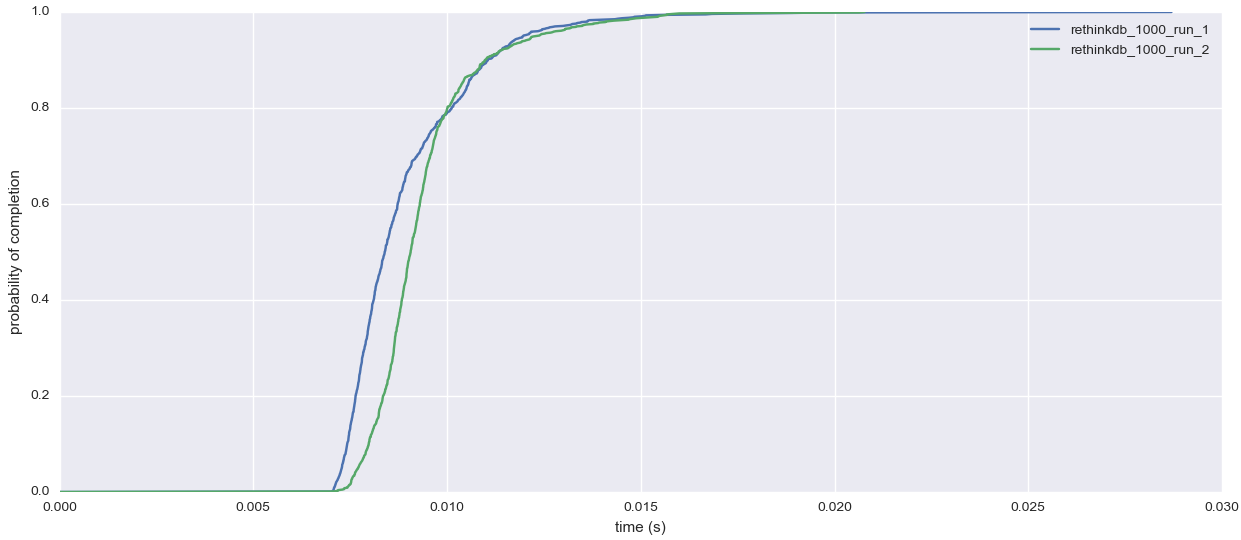
\includegraphics[width=0.8\paperwidth]{results_rethinkdb_1000_mass.png}}
  \caption{RethinkDB: 1000 run.}
\end{figure}

\begin{figure}[H]
  \makebox[\textwidth][c]{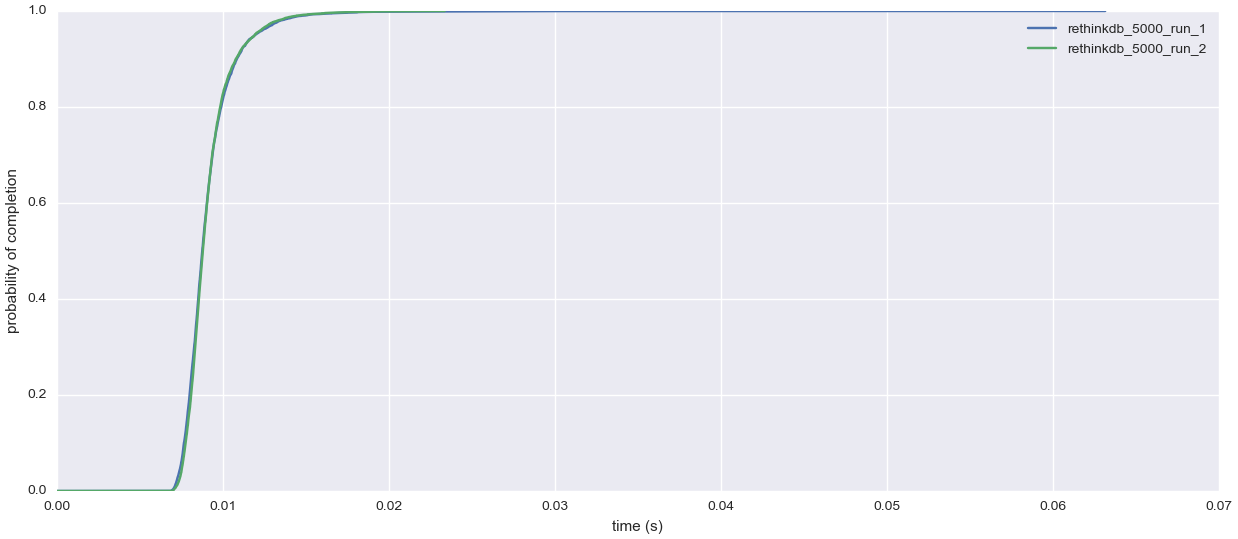
\includegraphics[width=0.8\paperwidth]{results_rethinkdb_5000_mass.png}}
  \caption{RethinkDB: 5000 run.}
  \label{rethinkdb_stable}
\end{figure}

\begin{figure}[H]
  \makebox[\textwidth][c]{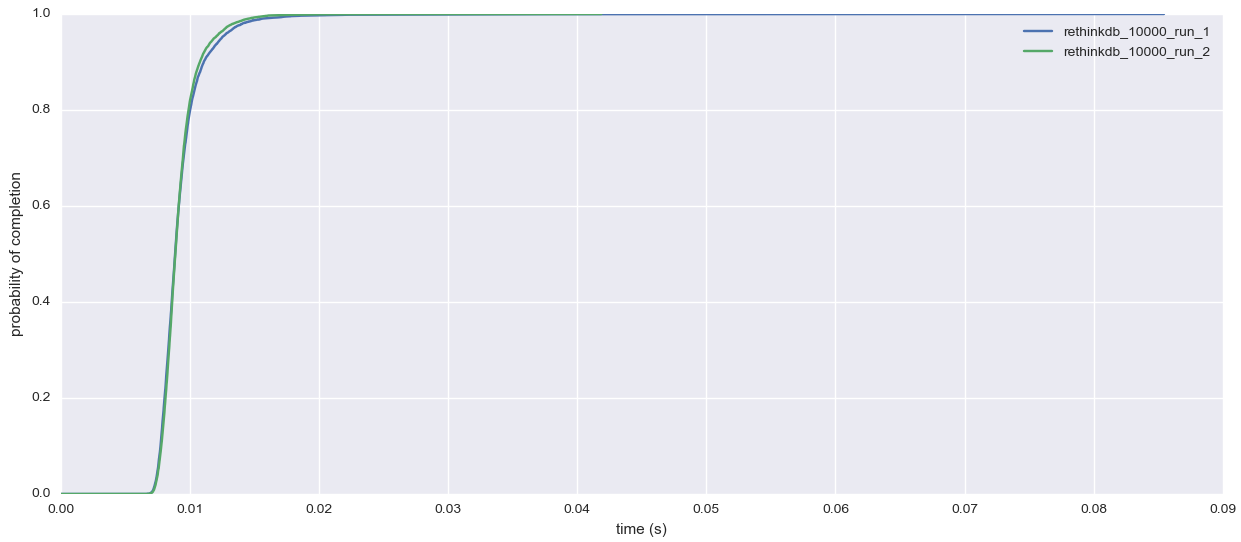
\includegraphics[width=0.8\paperwidth]{results_rethinkdb_10000_mass.png}}
  \caption{RethinkDB: 10000 run.}
\end{figure}

The parameter has been validated also on every other consensus algorithm. Figure \ref{paxos5000} shows the test on Multi-paxos.

\begin{figure}[H]
  \makebox[\textwidth][c]{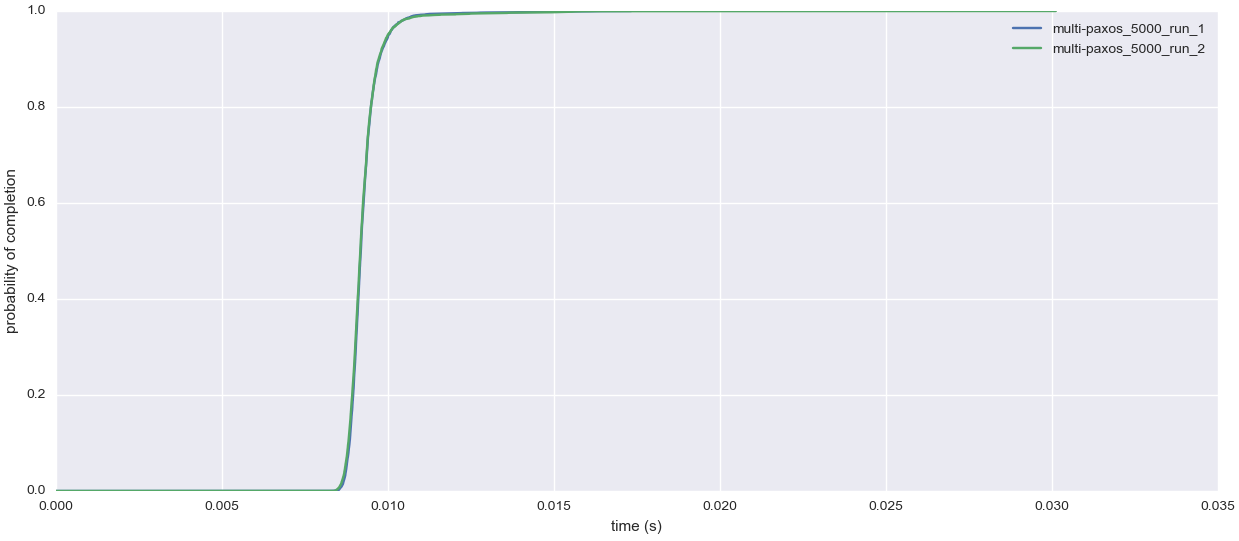
\includegraphics[width=0.8\paperwidth]{results_paxos_5000_mass.png}}
  \caption{Multi-Paxos: 5000 run.}
  \label{paxos5000}
\end{figure}

\section{Choosing the cluster size}
Another parameter to be fixed in advance has been the number of nodes composing the cluster. An upper bound of 8 has been set due to Compute Engine that doesn’t allow free-trial users to create more instances at the same time in the same region. Therefore, the value 5 has been chosen because it is reasonable enough for the majority of real distributed systems. Moreover, tests have been made to ensure that the performances on 5 nodes are not that far from the ones obtained on different size of the clusters. This has been investigated also for Multi-paxos, leading to very similar results. 

\section{Test suite description}
This section describes in depth each test in the suite. They can be divided into the following different main areas: gold standard, symmetric scenarios, asymmetric scenarios, Raft vs Paxos and Raft vs Raft.

\subsection{Gold standard}
This represents the baseline performance metric used as a guide to understand all the other results, providing insights on what to expect from every implementation. As explained before, these tests do not involve any change in the network layer.

\begin{figure}[H]
  \makebox[\textwidth][c]{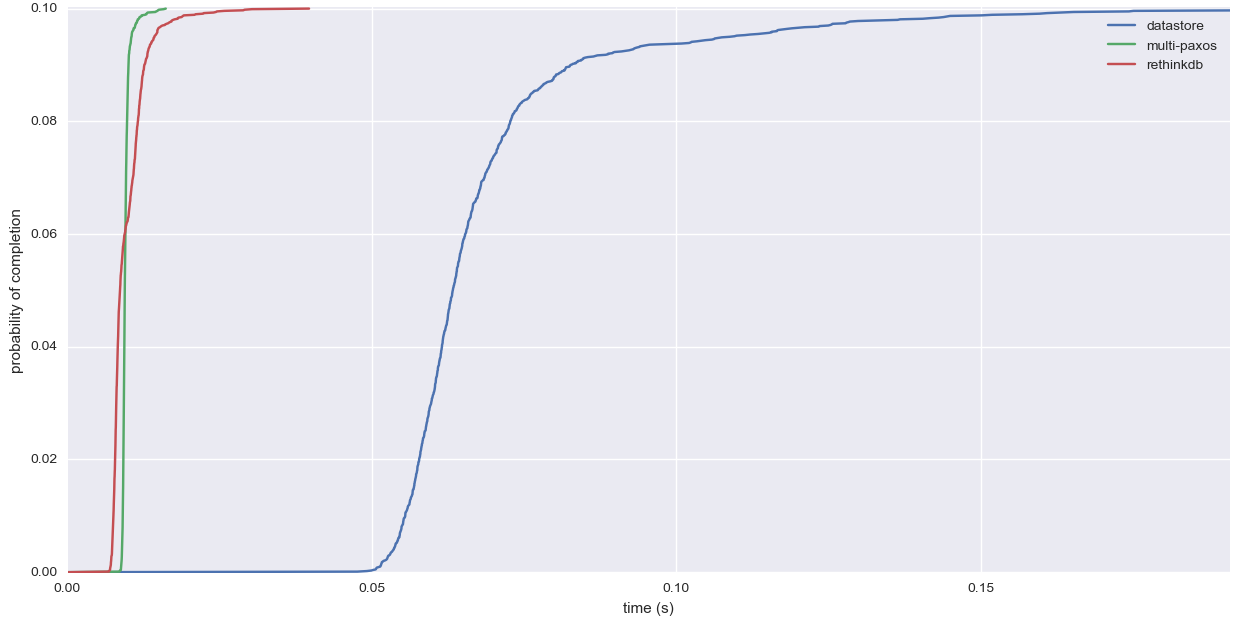
\includegraphics[width=0.8\paperwidth]{results_mass_3.png}}
  \caption{Datastore vs Multi-Paxos vs RethinkDB: cumulative density function comparison.}
\end{figure}

\begin{figure}[H]
  \makebox[\textwidth][c]{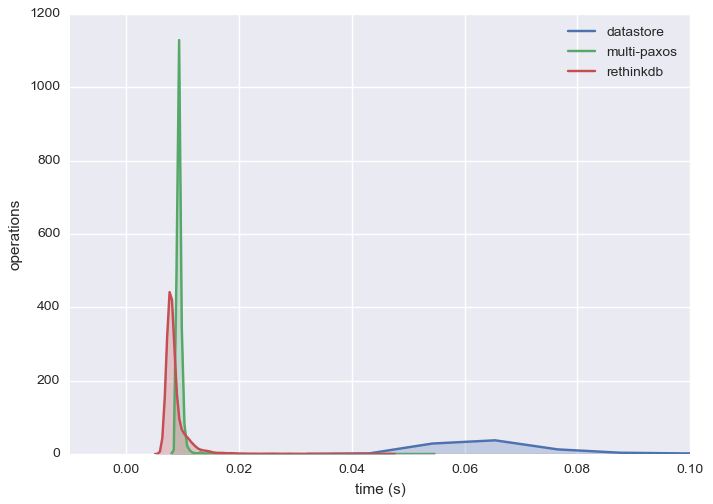
\includegraphics[width=0.6\paperwidth]{results_distribution_3.png}}
  \caption{Datastore vs Multi-Paxos vs RethinkDB: probability density function comparison.}
\end{figure}

The figures above show both the CDFs and the distributions functions of the chosen implementations. It is possible to notice how Datastore performs significantly worse than the other two algorithms and has the largest variance in the execution time. These results may be due to the fact that Datastore is not customizable by the user at will, implying that it is not possible neither to know the number of nodes the physical cluster is composed of nor to control the network traffic between them. Its execution time is approximately four time slower than the others, but it’s likely that the values stored on Datastore are replicated across Google data centers around the world on a huge amount of nodes.\\
A similar experiment has been executed in the pseudo-distributed mode. The results shown in figure \ref{local_standard} demonstrates how PySyncObj is significantly slower than every other implementations. Moreover, Multi-paxos seems to be slower than RethinkDB in this test, conversely to what shown in the previous experiment in the cloud. This is probably caused by the CPU-intensive nature of the implementation, whose effect is mitigated when nodes resides on physically different machines. On the contrary, on the local cluster all the nodes compete for the same CPU, thus mutually slowing themselves.

\begin{figure}[H]
  \makebox[\textwidth][c]{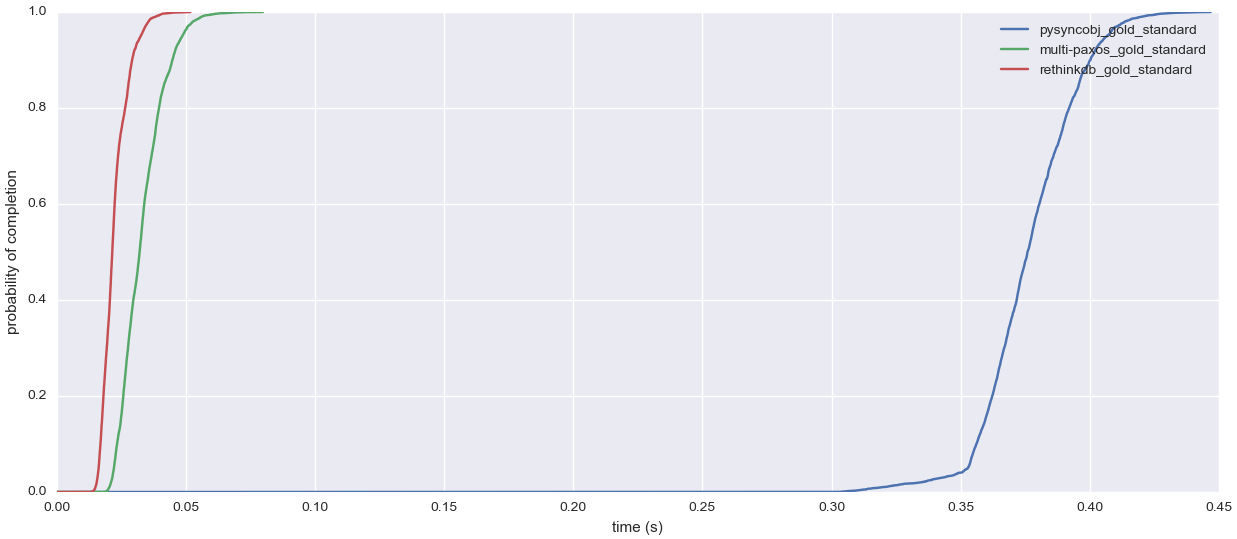
\includegraphics[width=0.8\paperwidth]{results_mass_4.png}}
  \caption{PySyncObj vs Multi-Paxos vs RethinkDB: cumulative density function comparison.}
  \label{local_standard}
\end{figure}

\begin{figure}[H]
  \makebox[\textwidth][c]{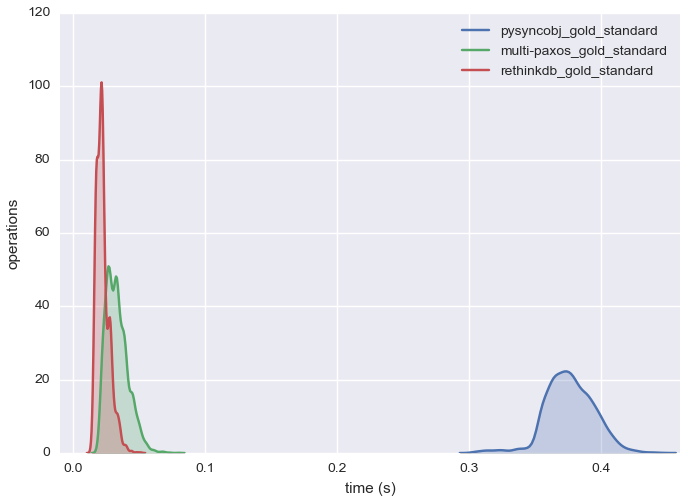
\includegraphics[width=0.6\paperwidth]{results_distribution_4.png}}
  \caption{PySyncObj vs Multi-Paxos vs RethinkDB: probability density function comparison.}
\end{figure}

\subsection{Symmetric scenarios}
These tests shows how the system performance degrades while increasing problems on the network in a homogeneous manner. They have been specifically crafted to give the consensus algorithm hard times in replicating data between the nodes. Every distributed algorithm relying upon message passing for communication should be affected by these changes. The completed tests are the following:

\begin{itemize}
    \item packet delay: every node in the cluster transmits with a certain delay its packets, both ingoing and outgoing. The tested delay are 10 ms, 15 ms and 20 ms.

    \begin{figure}[H]
      \makebox[\textwidth][c]{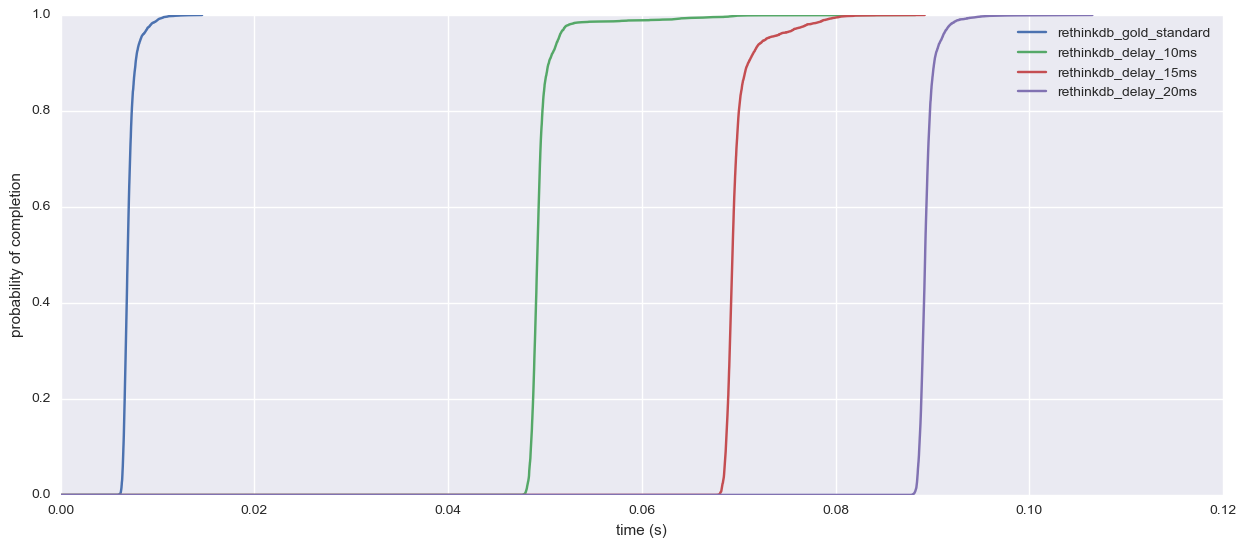
\includegraphics[width=0.8\paperwidth]{results_delay_mass_5.png}}
      \caption{RethinkDB: cumulative density function with delay.}
      \label{delay}
    \end{figure}

    \begin{figure}[H]
      \makebox[\textwidth][c]{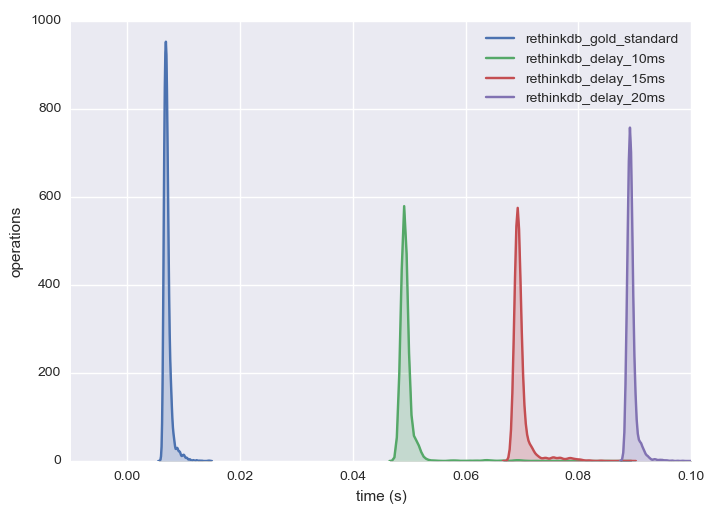
\includegraphics[width=0.6\paperwidth]{results_delay_distribution.png}}
      \caption{RethinkDB: probability density function with delay.}
      \label{delay_distr}
    \end{figure}

    \item packet loss: every node in the cluster loses a certain percentage of packets, both ingoing and outgoing. The tested percentages are \(2\%\), \(4\%\) and \(6\%\) with a uniform distribution.

    \begin{figure}[H]
      \makebox[\textwidth][c]{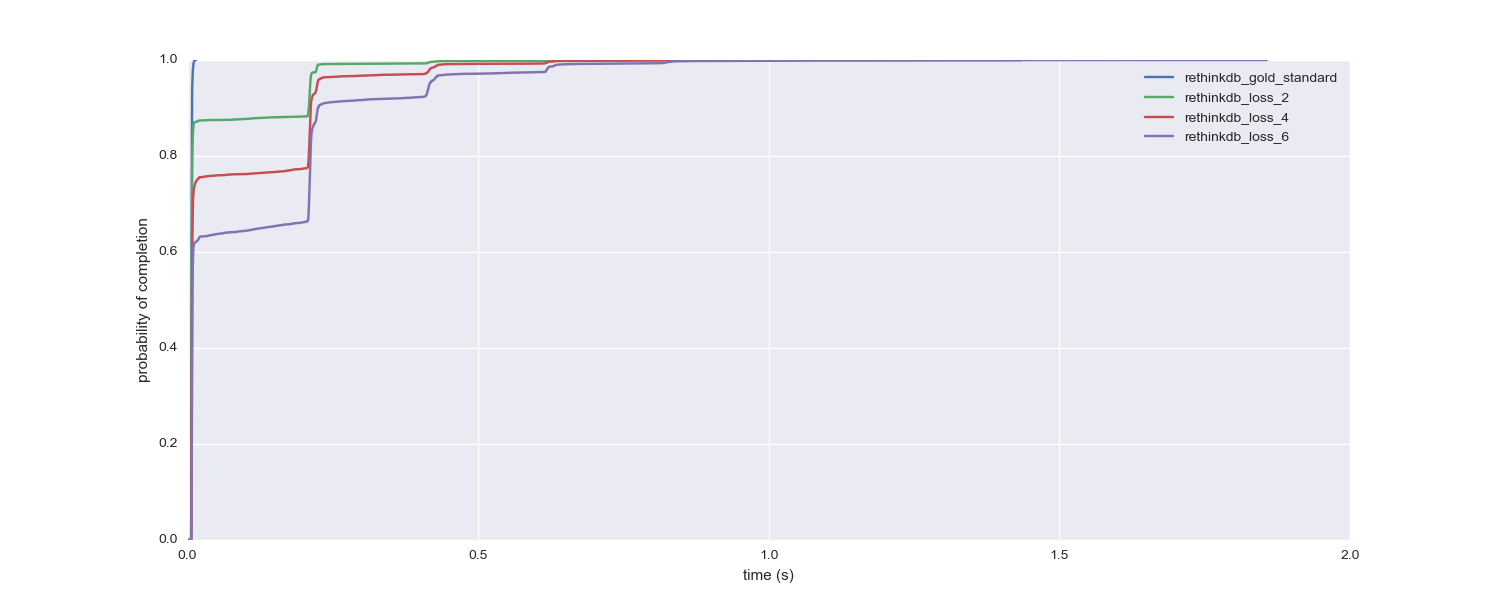
\includegraphics[width=0.8\paperwidth]{results_loss_mass.png}}
      \caption{RethinkDB: cumulative density function with loss.}
      \label{loss}
    \end{figure}

    \item packet corruption: every node corrupts a certain amount of packets, both ingoing and outgoing. The tested percentages are \(2\%\), \(4\%\) and \(6\%\) with a uniform distribution.

    \begin{figure}[H]
      \makebox[\textwidth][c]{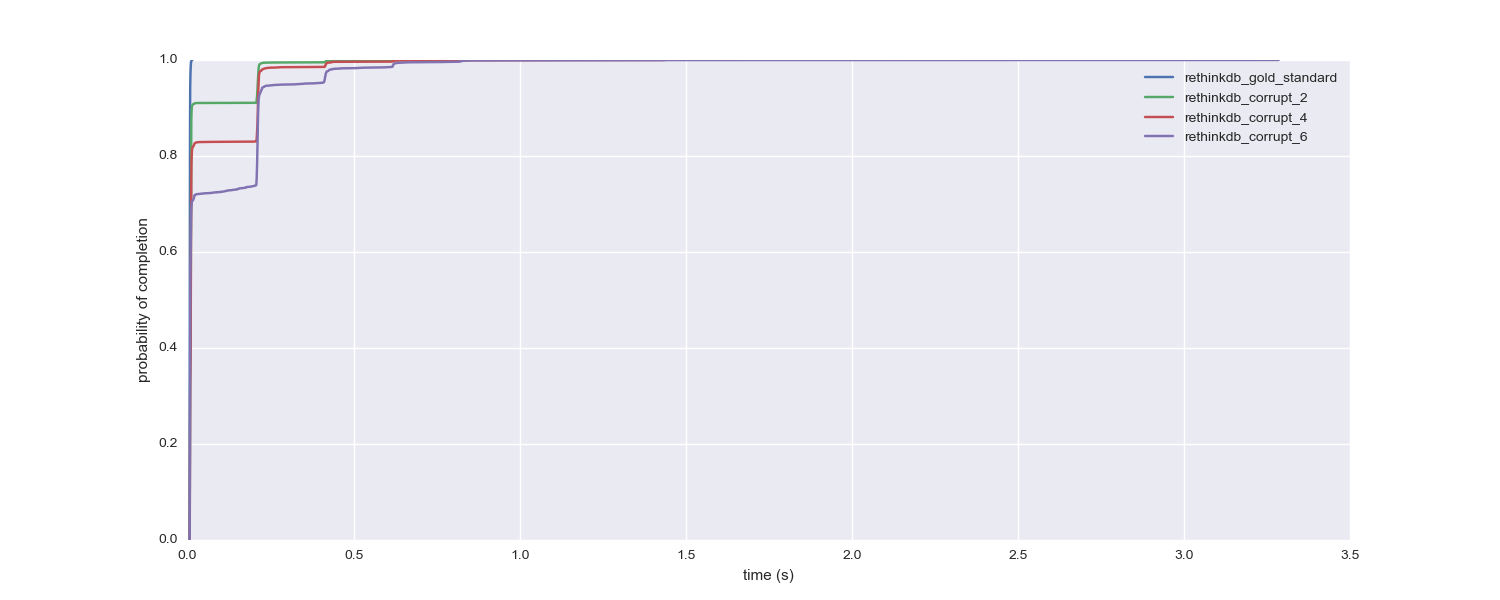
\includegraphics[width=0.8\paperwidth]{results_corruption_mass.png}}
      \caption{RethinkDB: cumulative density function with packet corruption.}
      \label{corruption}
    \end{figure}

    \item packet inversion: every node randomly reorders \(50\%\) of the packets, both ingoing and outgoing and sends the other half with a certain delay. The chosen delays are 10 ms and 20 ms.

    \begin{figure}[H]
      \makebox[\textwidth][c]{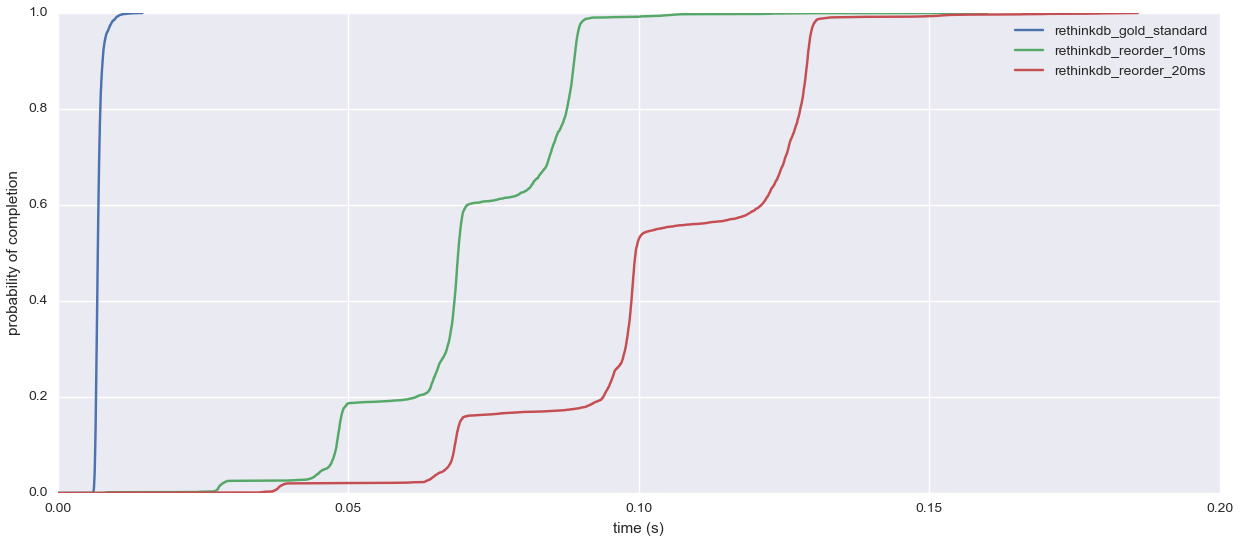
\includegraphics[width=0.8\paperwidth]{results_reorder_mass.png}}
      \caption{RethinkDB: cumulative density function with packet reordering.}
    \end{figure}
\end{itemize}

In the figures \ref{delay}, \ref{loss} and \ref{corruption} the trend of the CDFs clearly shows how introducing these network issues influences the time the system needs to reach consensus in a proportional manner. This effect can be seen by looking at the shift of the lines along the x axis towards higher values of elapsed time. The proportionality factor can provide some insights on the number of messages that are exchanged by RethinkDB to reach consensus. As it can be seen in the figure \ref{delay_distr}, with a 10 ms delay the consensus is reached on average in 50 ms. By increasing the delay of only 5 ms, the consensus time increases to 70 ms. The average number of sequential messages exchanged by RethinkDB can be thus computed with the following formula:

\begin{align*}
  0.50 - 0.10*n &= 0.70 - 0.15*n \\
  n &= 4
\end{align*}

The packets loss graph shows different information. The first gap underlines the effect of one packet loss on the consensus algorithm. The height of each gap represents the probability of not losing more than one packet and it represents an index of the minimum number of messages (not necessarily in sequence) that the underlying algorithm needs to exchange to reach consensus. In fact, increasing loss percentages decreases the probability of reaching consensus (red and purple lines). The second gap, similarly, represents the loss of two packets and so do the successive ones. The distance on the x axis between two gaps represents the time that RethinkDB takes to recover from a packet loss and it is constant on each gap (\(\sim0.2s\)).\\
A similar behaviour can be seen on the packet corruption graph. The main difference from the packet loss is that corruption seems to affect less the protocol, since consensus probabilities are slightly higher. This trend can be due to the fact that one bit corruption has a non-zero probability of leaving the TCP packet intact from an application level point of view.\\
The reordering graph, on the other hand, shows a different behaviour which seems to be the combination of both packets loss and delay.

\subsection{Asymmetric scenarios}
These tests show how the system performance degrades when the network faces problems on a specific subset of nodes. Adversarial network conditions have been applied only to some nodes to model new network situations, common in distributed systems. The tests that have been completed are the following:

\begin{itemize}
    \item faulty network cards: 1 random bit of ingoing and outgoing packets gets corrupted with a probability of 0.1. One at a time, every node of the cluster suffers this condition.

    \begin{figure}[H]
      \makebox[\textwidth][c]{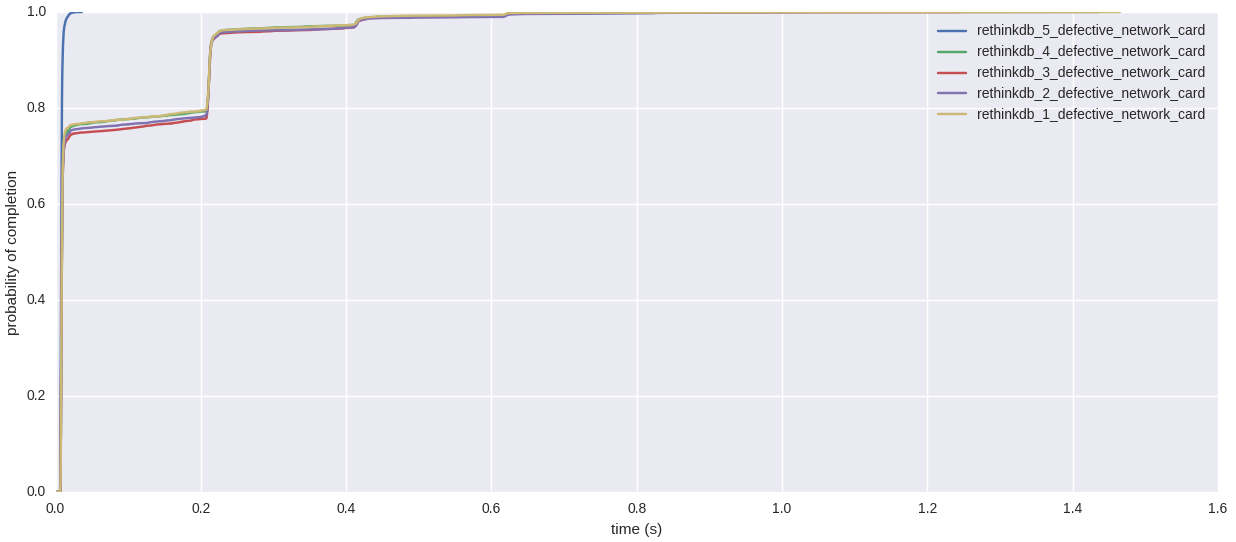
\includegraphics[width=0.8\paperwidth]{results_rethinkdb_broken_network_card_mass.png}}
      \caption{RethinkDB: cumulative density function with broken network cards.}
      \label{broken_nic}
    \end{figure}

    \item partitions: some links that connect a group of the nodes in the cluster to the others are slowed down. This situation simulate a distributed system whose nodes are logically partitioned into two different regions. In this way the intra-partition communication is slow, but, at the same time, the inter-partition communication is left unchanged.

    \begin{figure}[H]
      \makebox[\textwidth][c]{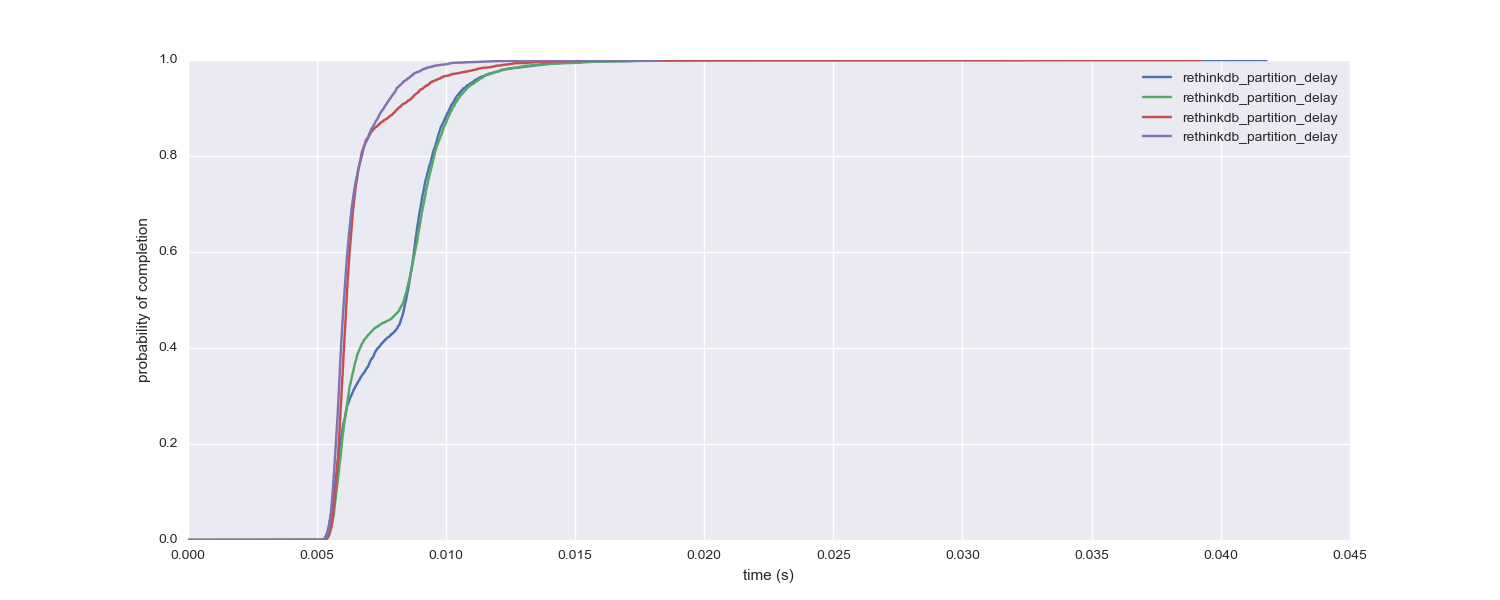
\includegraphics[width=0.8\paperwidth]{results_rethinkdb_slow_links_between_regions_mass.png}}
      \caption{RethinkDB: cumulative density function with partitions.}
      \label{partitions}
    \end{figure}
\end{itemize}

The results in figure \ref{broken_nic} shows two different behaviours. If the node having the problem is one which is not necessarily involved in the majority to reach consensus, the consequences are negligible (blue curve). On the other hand, if the faulty network card is the one of a node which is actually needed to obtain consensus, the performances deteriorate (all the other lines).\\
figure \ref{partitions} explains how the Raft algorithm responds to a logically-partitioned cluster with groups made of 2 and 3 nodes respectively. More in detail:

\begin{itemize}
    \item if the leader and a majority of the nodes are together, the algorithm is not delayed at all, since nobody in this partition needs to communicate with another node through a slow link. This situation is represented by the purple and the red lines on the left side.
    \item if the leader needs to contact any node afflicted by a slow link, it has to wait for him to respond and the overall performances are clearly worse (green and blue lines on the right). 
\end{itemize}

\subsection{Raft vs Paxos}
This test is thought to compare the two consensus algorithms and show which of them suffers more packets delay, which is probably the most frequent issues on real systems.

\begin{figure}[H]
  \makebox[\textwidth][c]{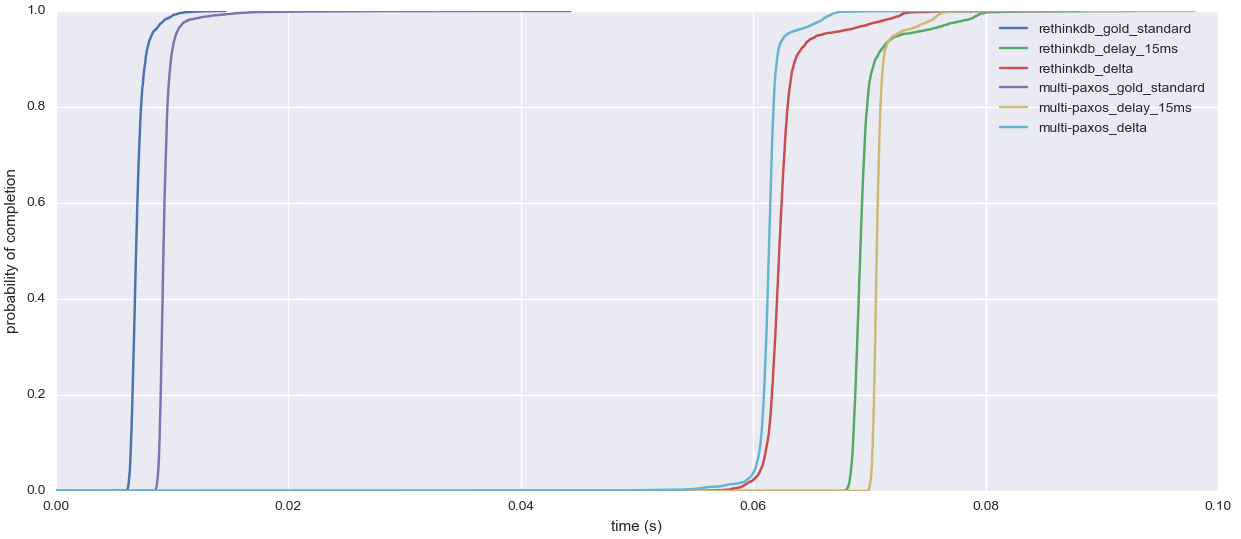
\includegraphics[width=0.8\paperwidth]{results_delay_mass_7.png}}
  \caption{RethinkDB vs Multi-Paxos: cumulative density function comparison with delay.}
\end{figure}

The figure above illustrates how Multi-paxos performs slightly better than RethinkDB if the delay is quite small (15 ms). This can be easily noticed by looking at the two curves in the middle, showing the difference between the gold standards and the delayed executions, where Multi-paxos (light blue) is on the left with respect to RethinkDB (red).

\subsection{Raft vs Raft}
Different implementations relying upon the same consensus algorithms are compared in order to demonstrate how RethinkDB clearly outperforms PySyncObj. In this way it is possible to see how a commercial product is orders of magnitude better than its counterpart from any point of view.

\begin{figure}[H]
  \makebox[\textwidth][c]{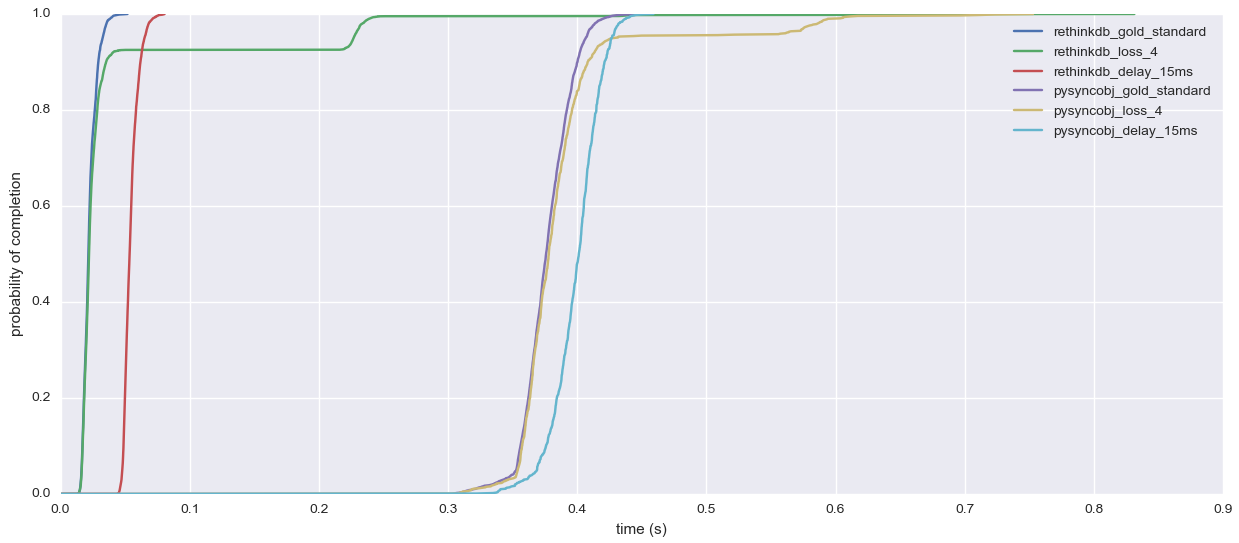
\includegraphics[width=0.8\paperwidth]{results_mass_raft.png}}
  \caption{RethinkDB vs PySyncObj: cumulative density function comparison with delay and loss.}
\end{figure}